\section{Generating training samples}
\label{sec: generating_training}
\cutsection

In this section we present our method for rapidly generating labeled training samples.

To rapidly generate training samples, we use a color glove that has a different color for each area of interest. We can present the glove to the camera and extract regions of a specific color using \textbf{RGB camera} and label the \textbf{corresponding depth pixel} appropriately. Examples of gloves we used in our experiments are shown in figure~\ref{fig:gloves}.

\begin{figure}
\begin{center}
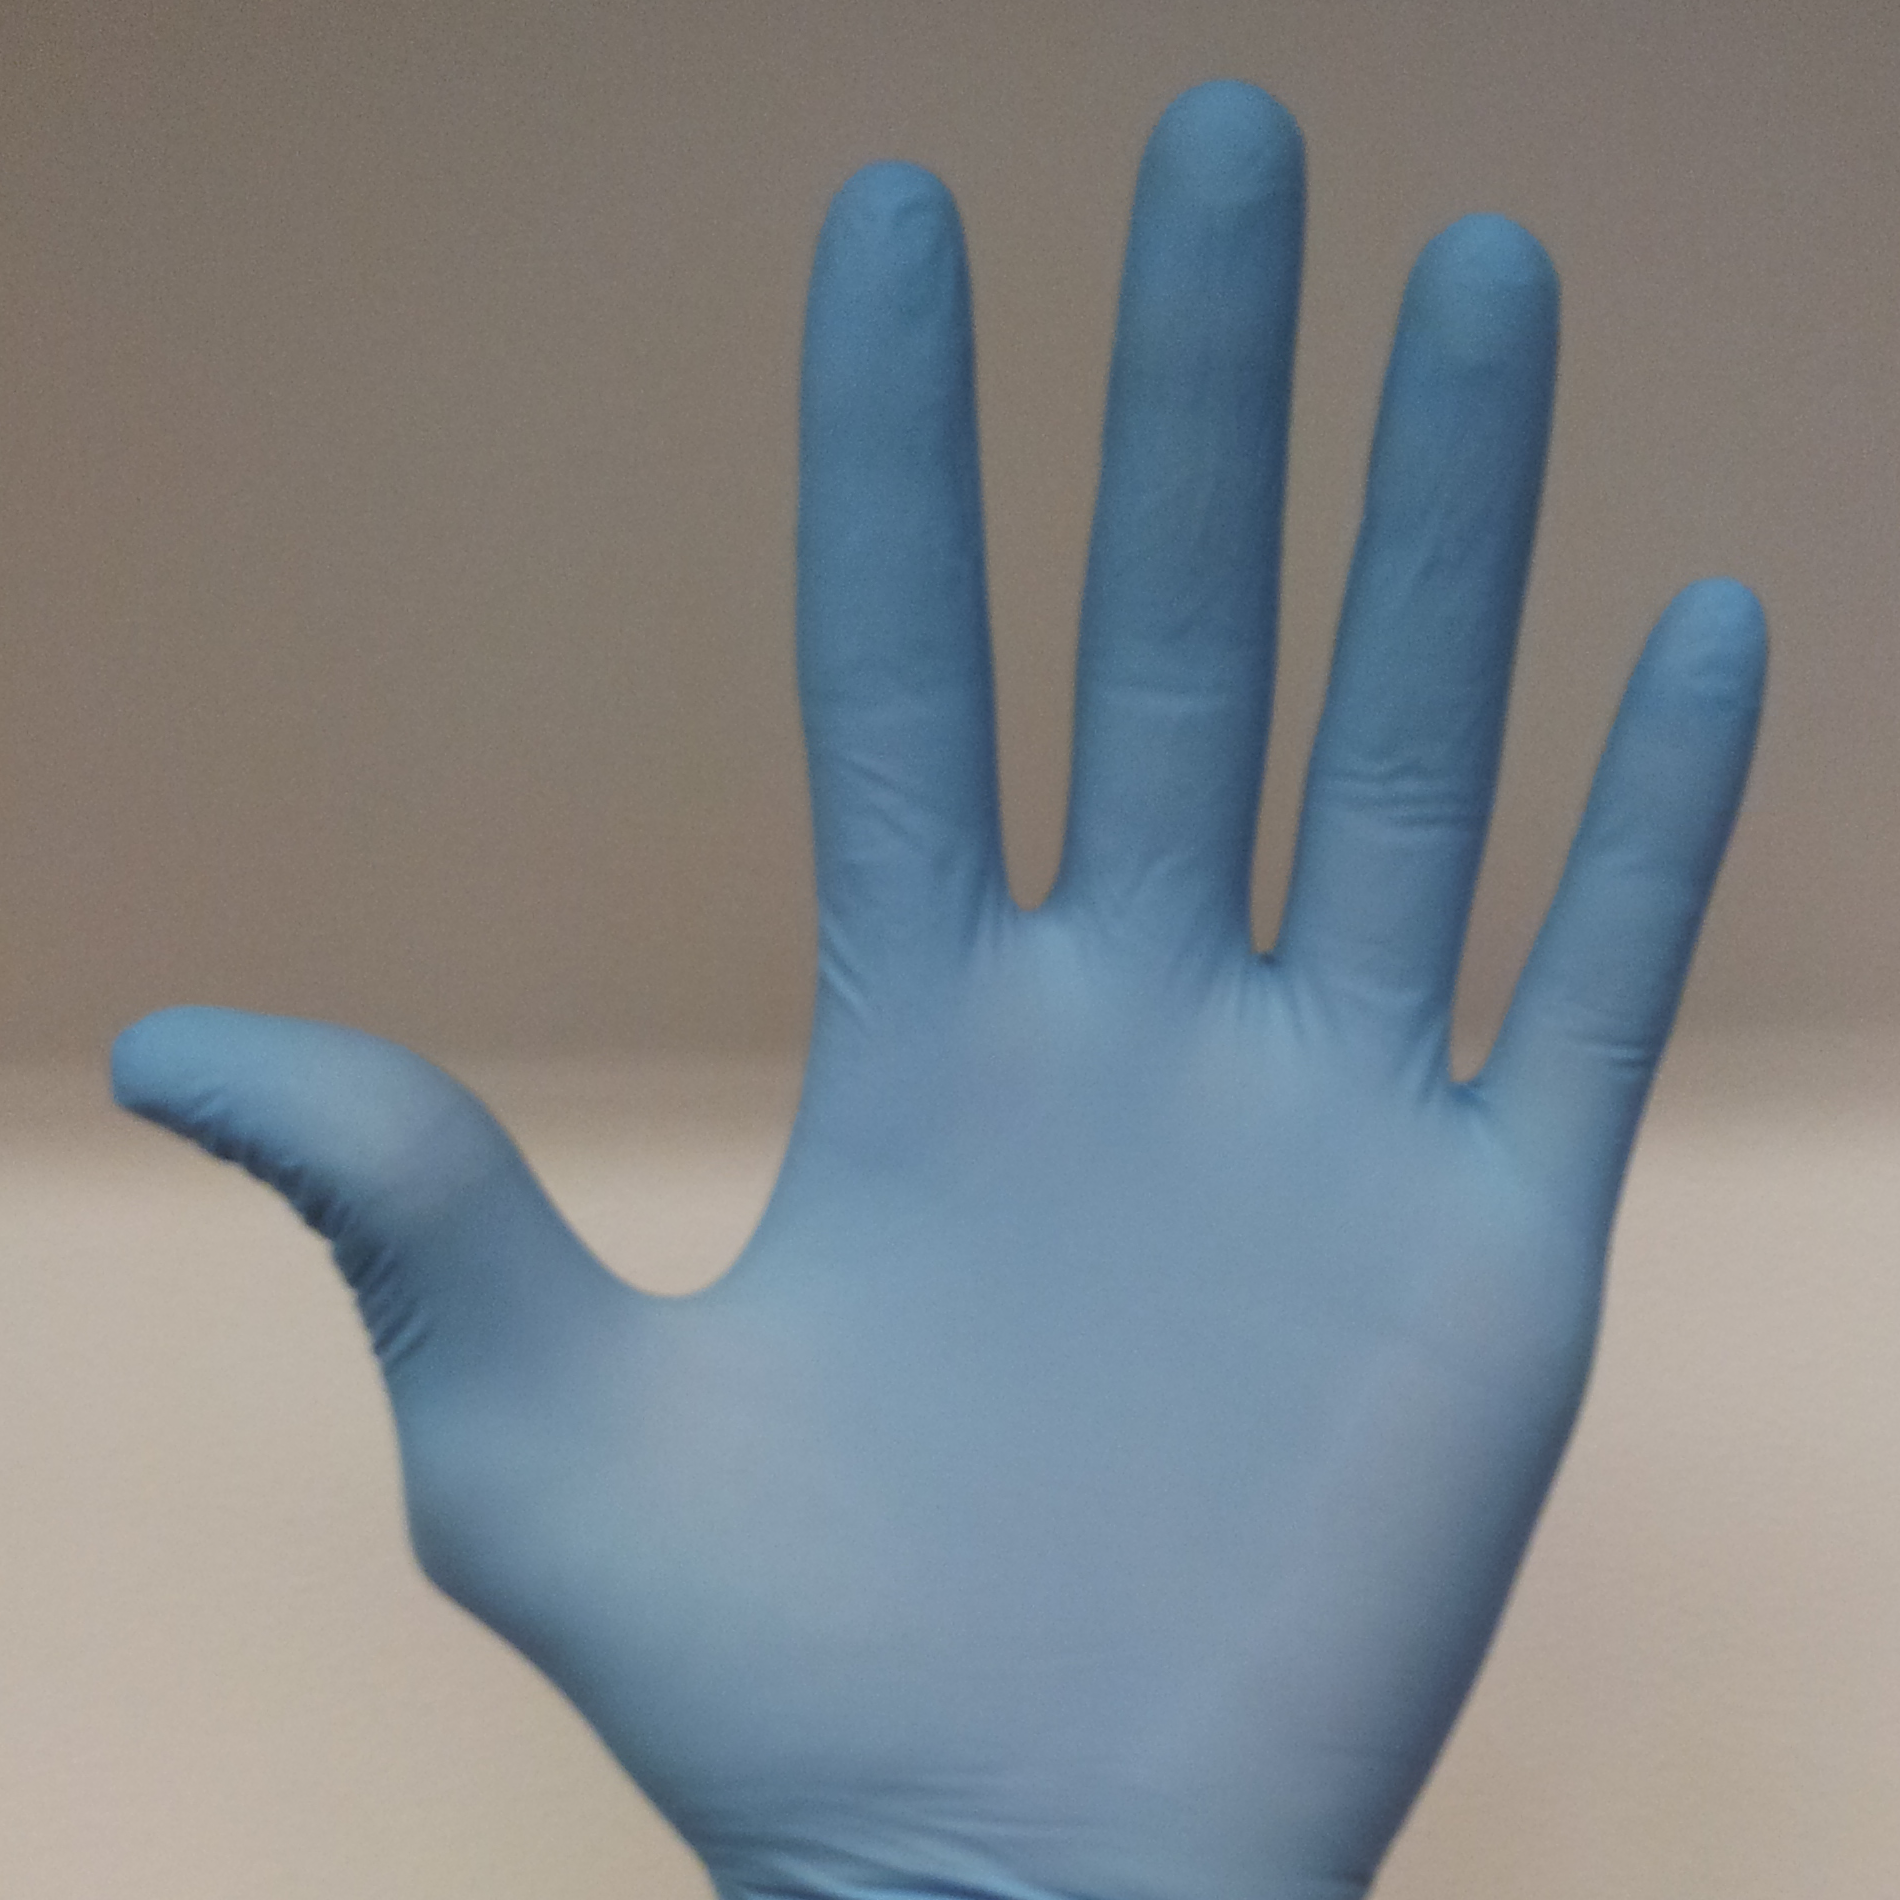
\includegraphics[width=0.23 \textwidth]{fig/blueglove.png}
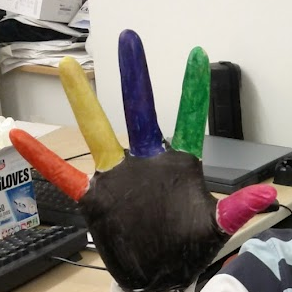
\includegraphics[width=0.23 \textwidth]{fig/colorglove.png}
\end{center}
\caption{Two differently colored gloves we used in rapidly generating labeled training samples. For the multicolored glove, we had to ensure the colors were different enough to be easily recognized by the RGB camera.}
\label{fig:gloves}
\end{figure}

\begin{figure}
\begin{center}

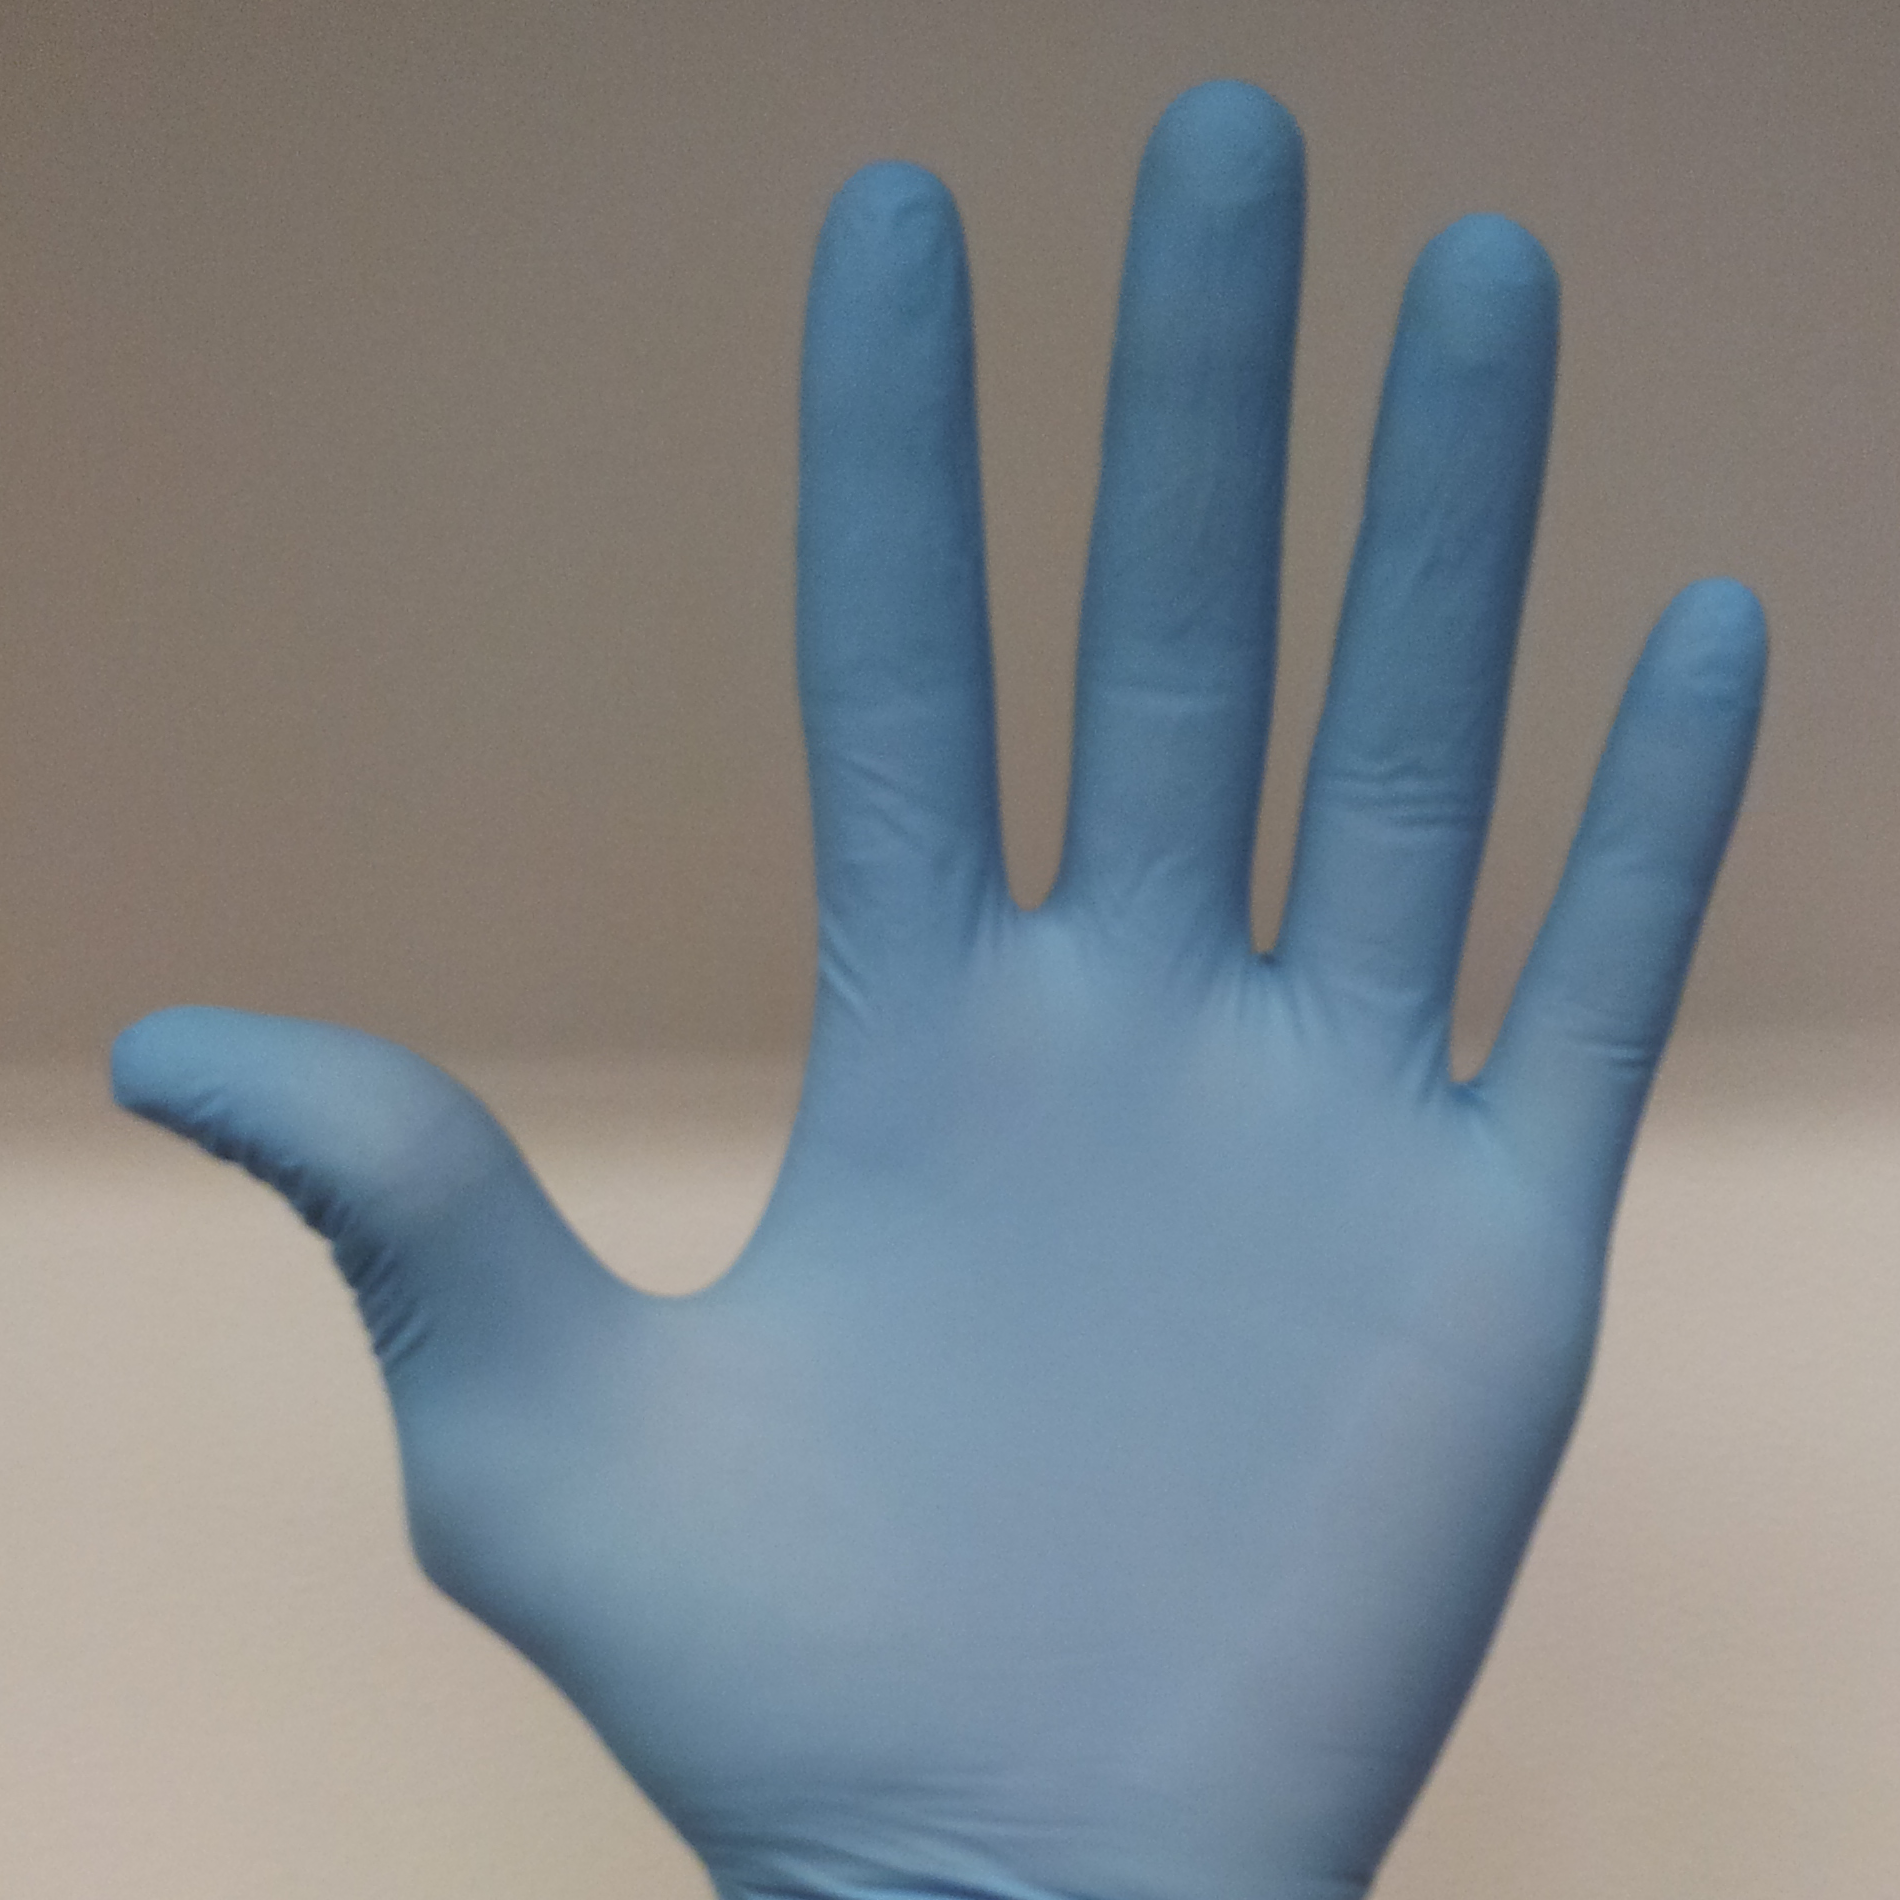
\includegraphics[width=0.11 \textwidth]{fig/gesture1.png}
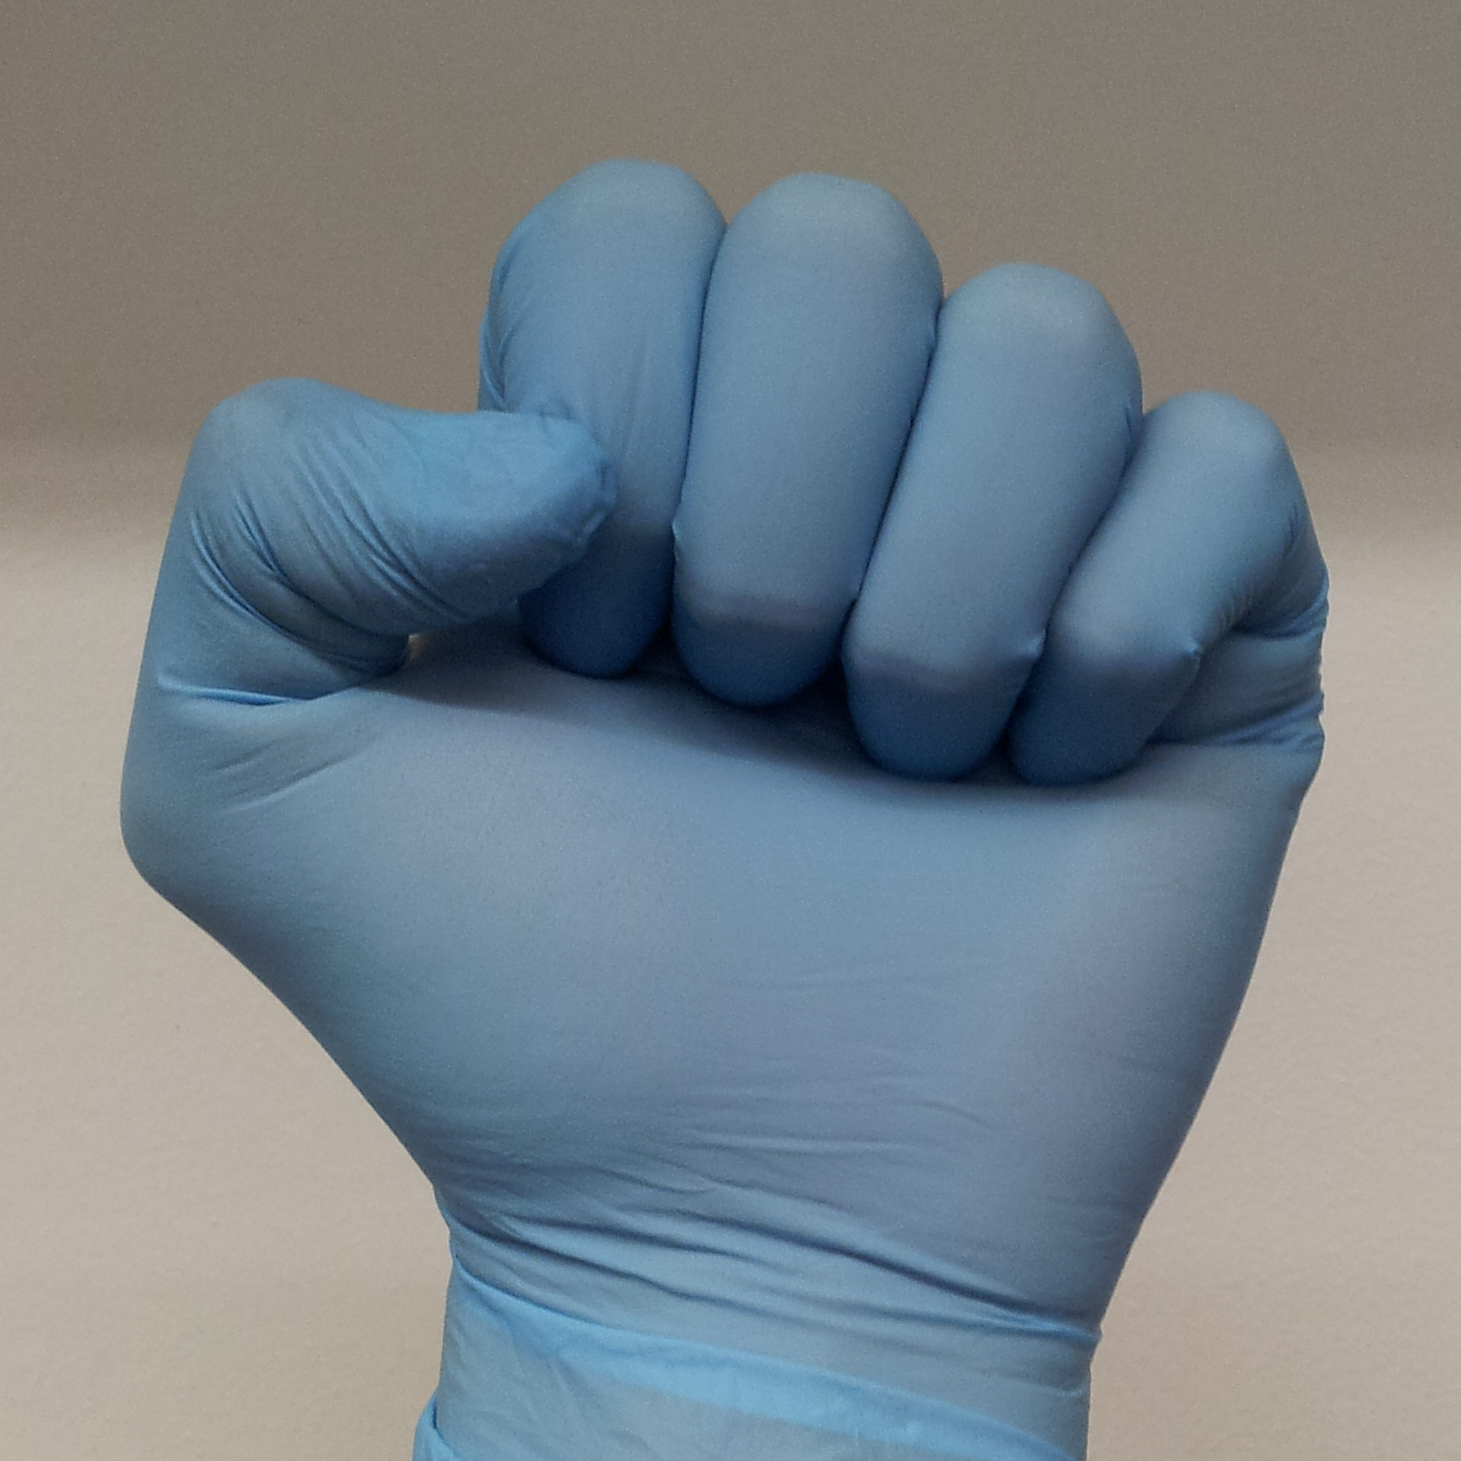
\includegraphics[width=0.11 \textwidth]{fig/gesture2.png}
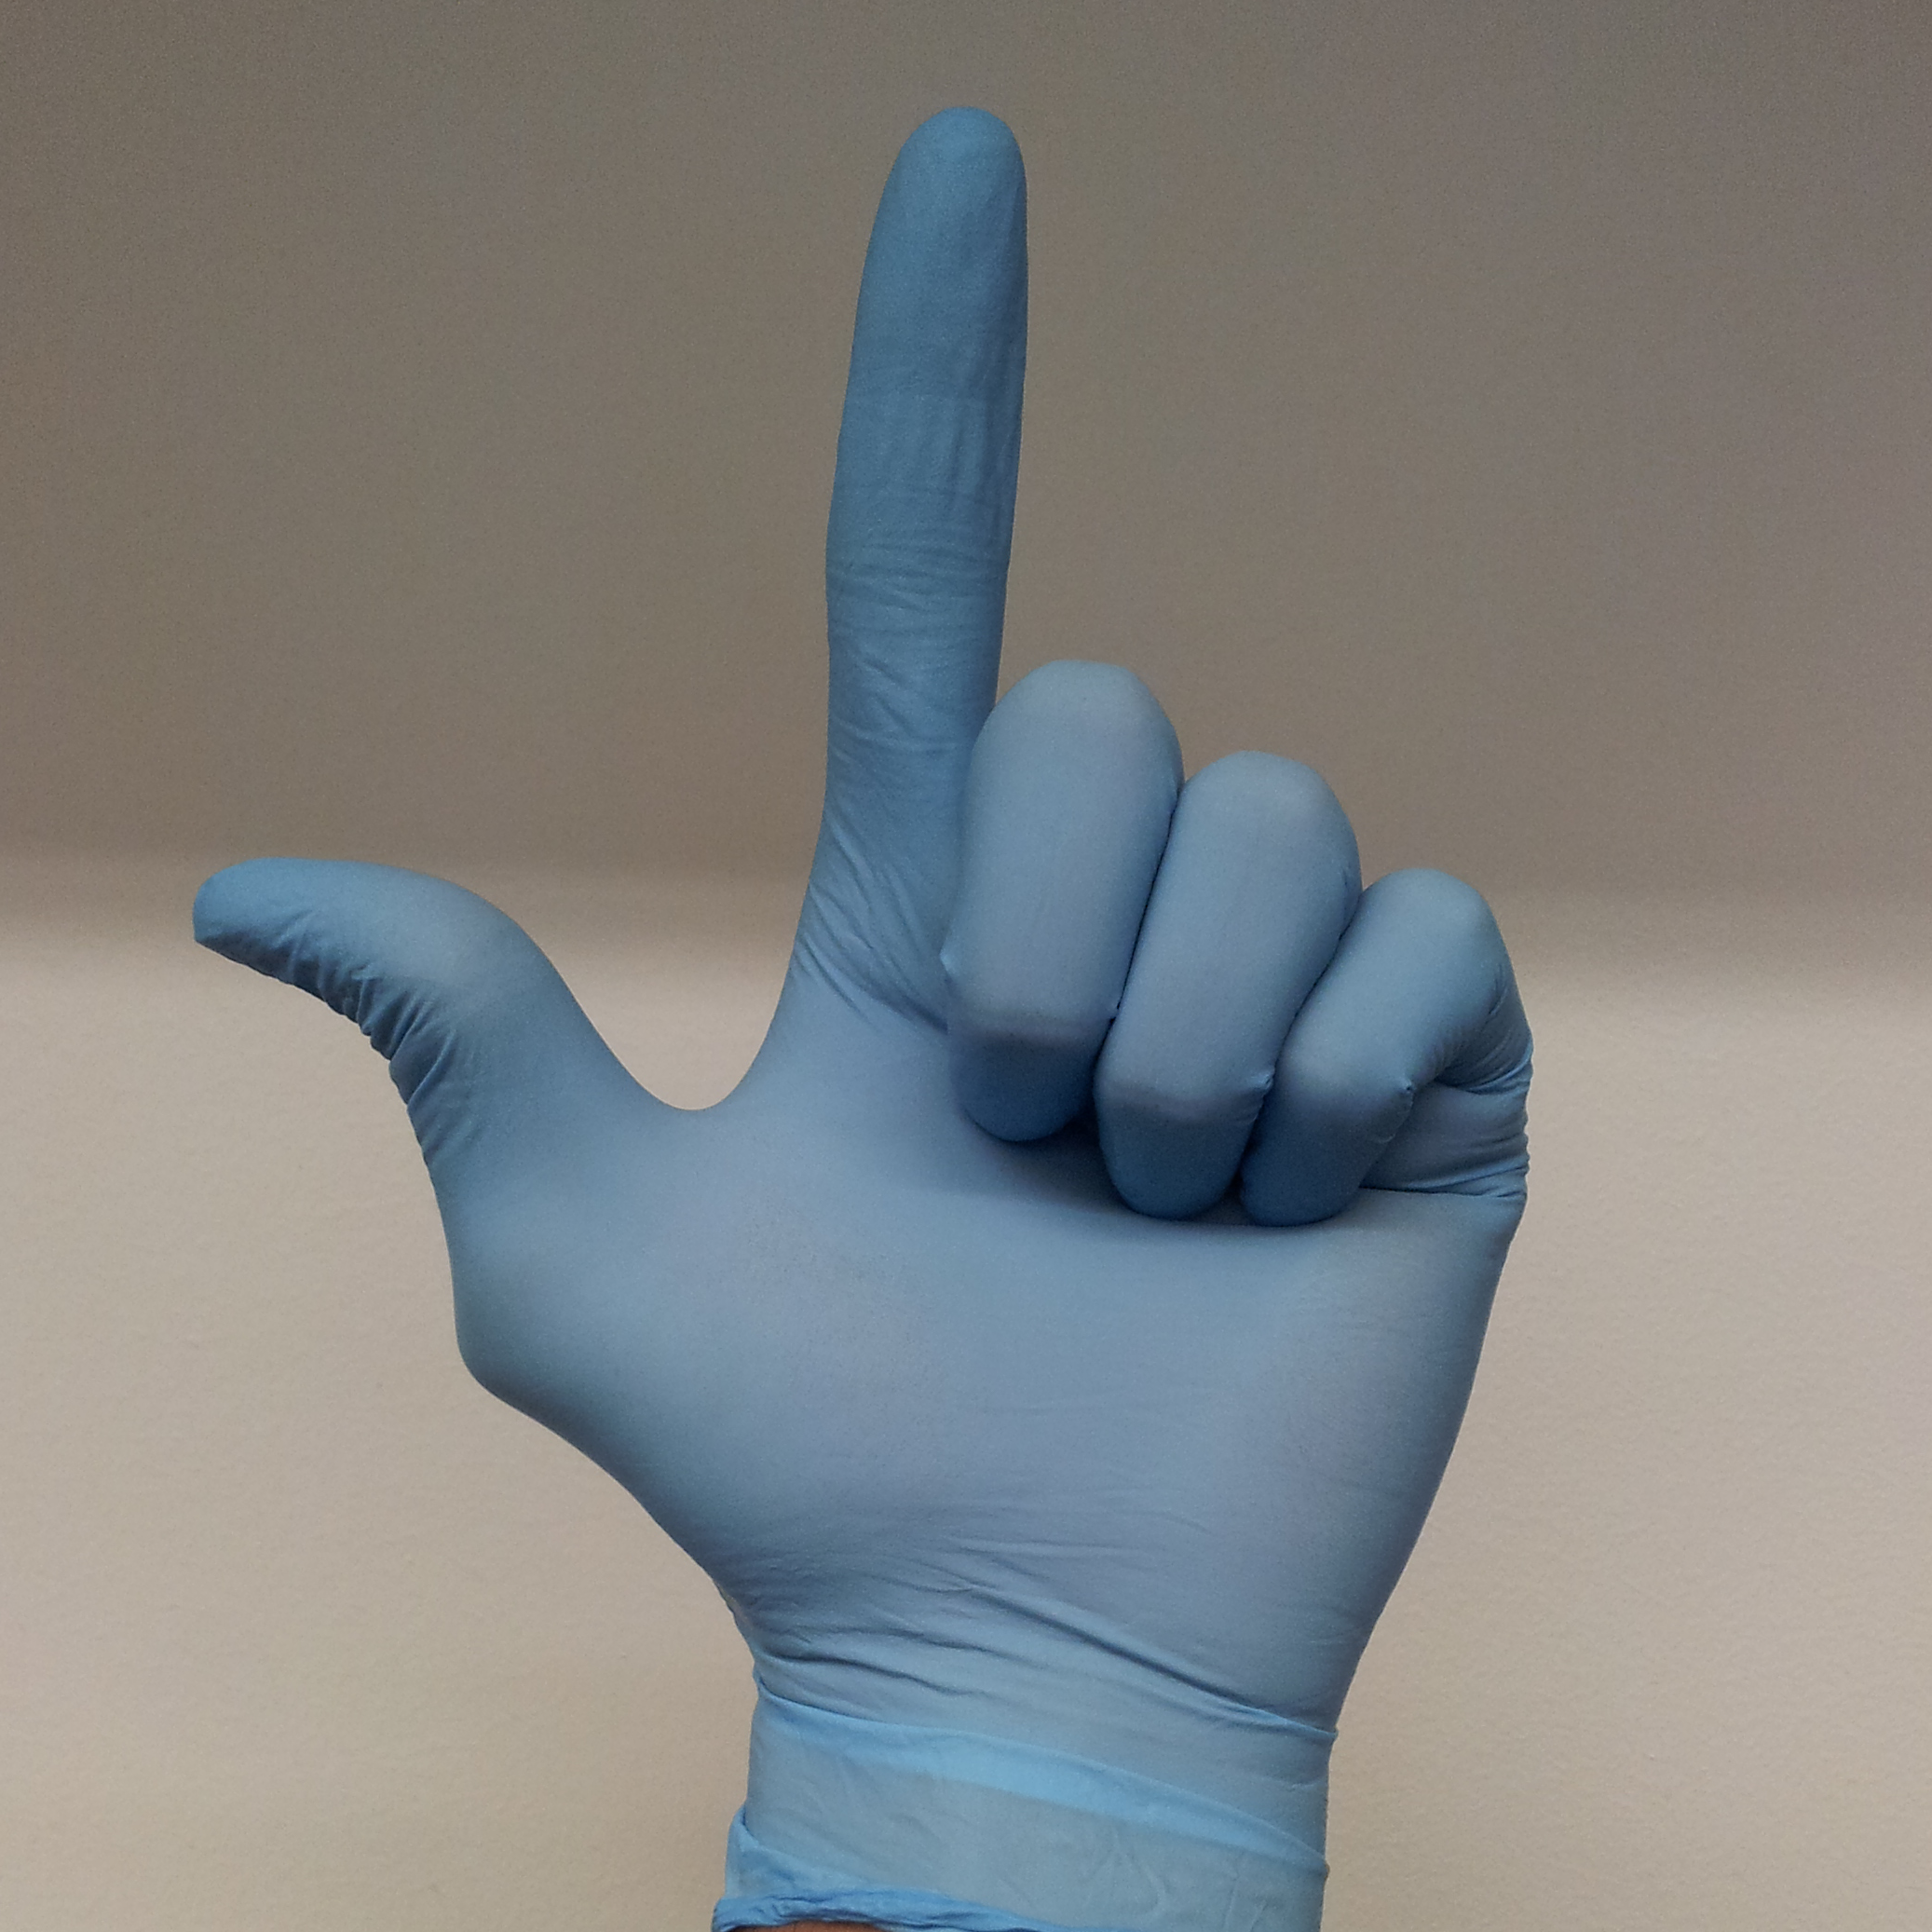
\includegraphics[width=0.11 \textwidth]{fig/gesture3.png}
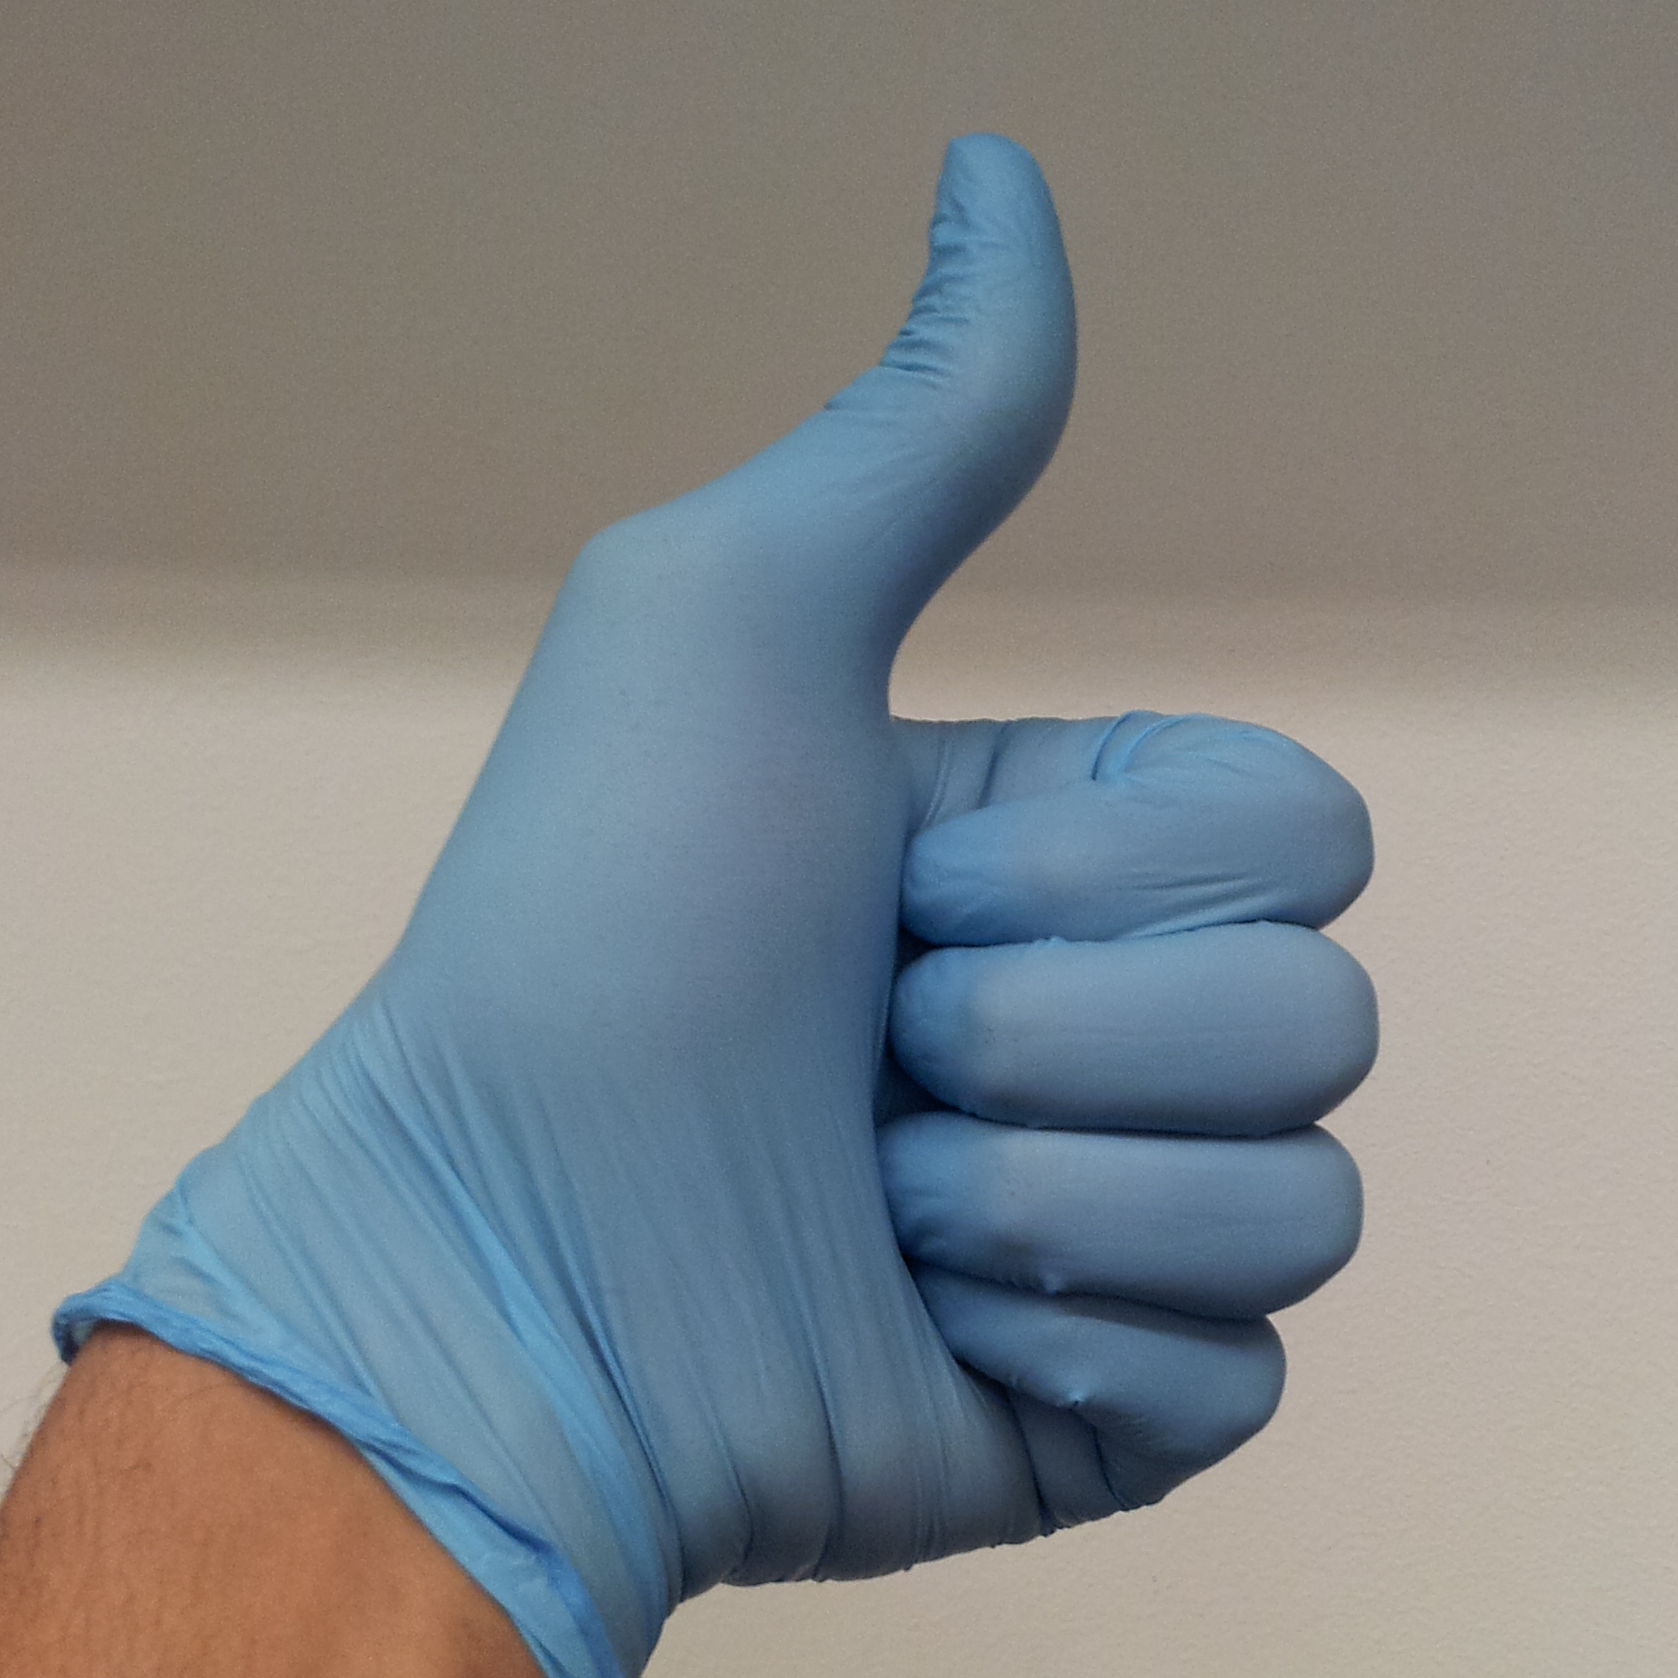
\includegraphics[width=0.11 \textwidth]{fig/gesture4.png}

%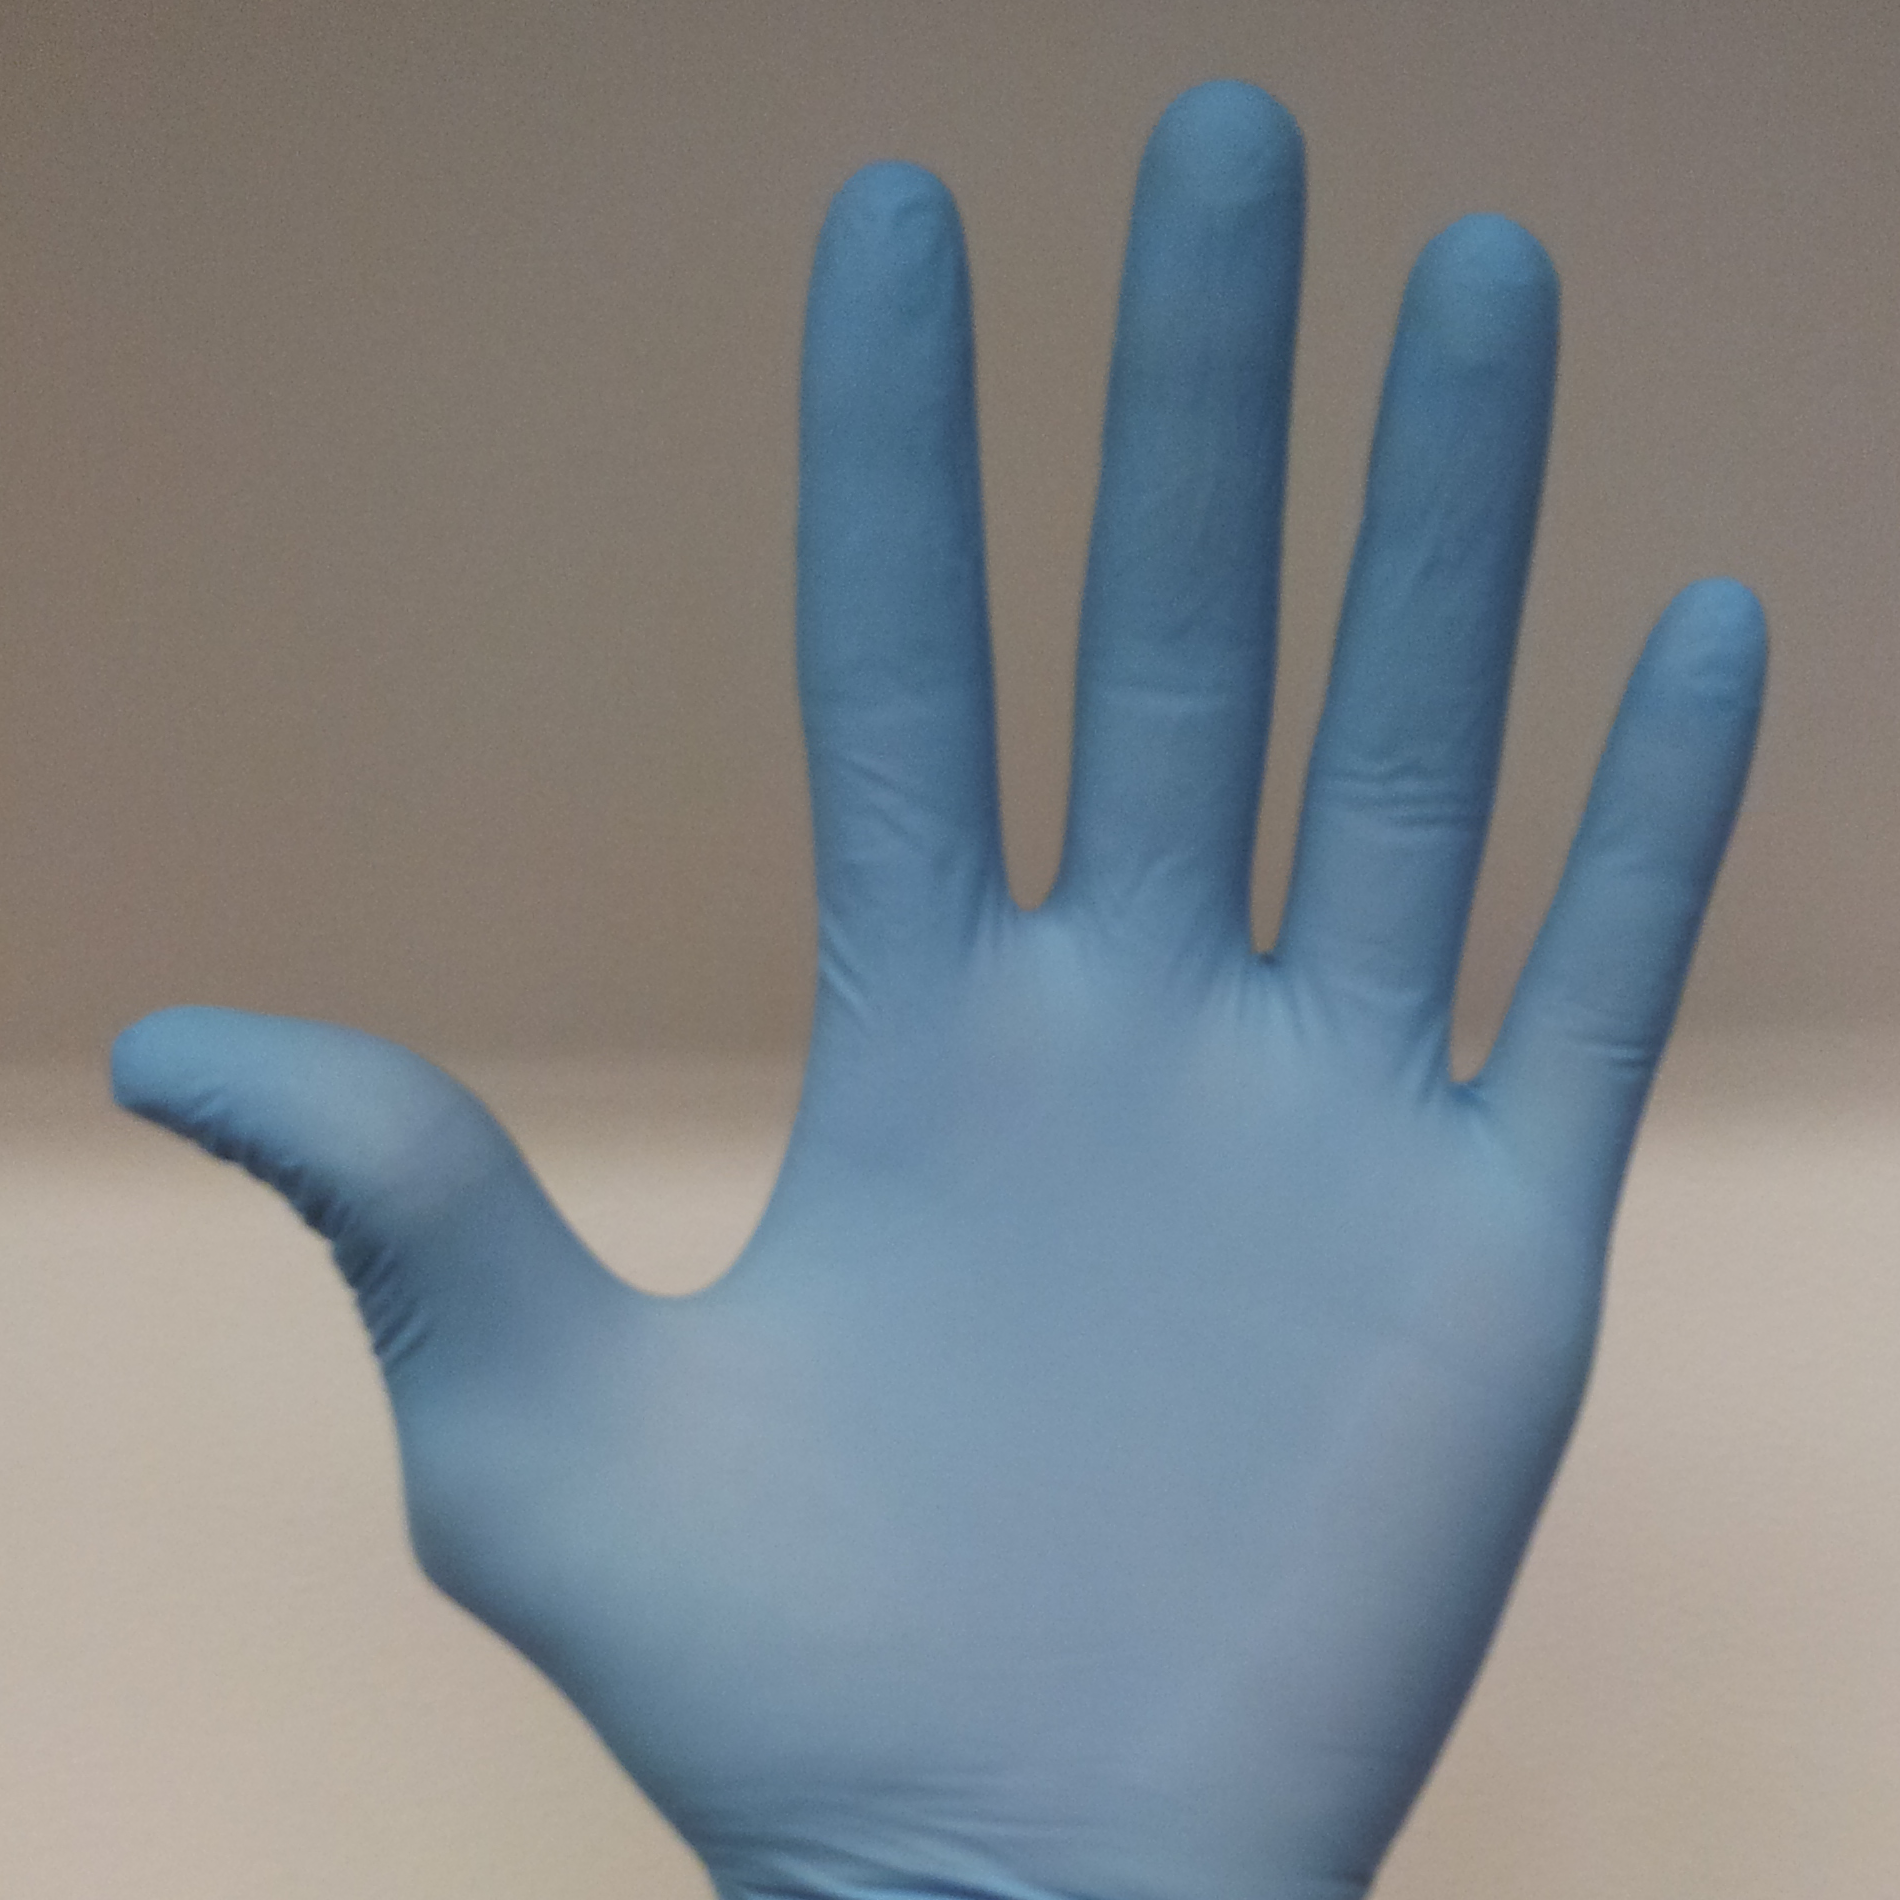
\includegraphics[width=0.23 \textwidth]{fig/gesture1.png}
%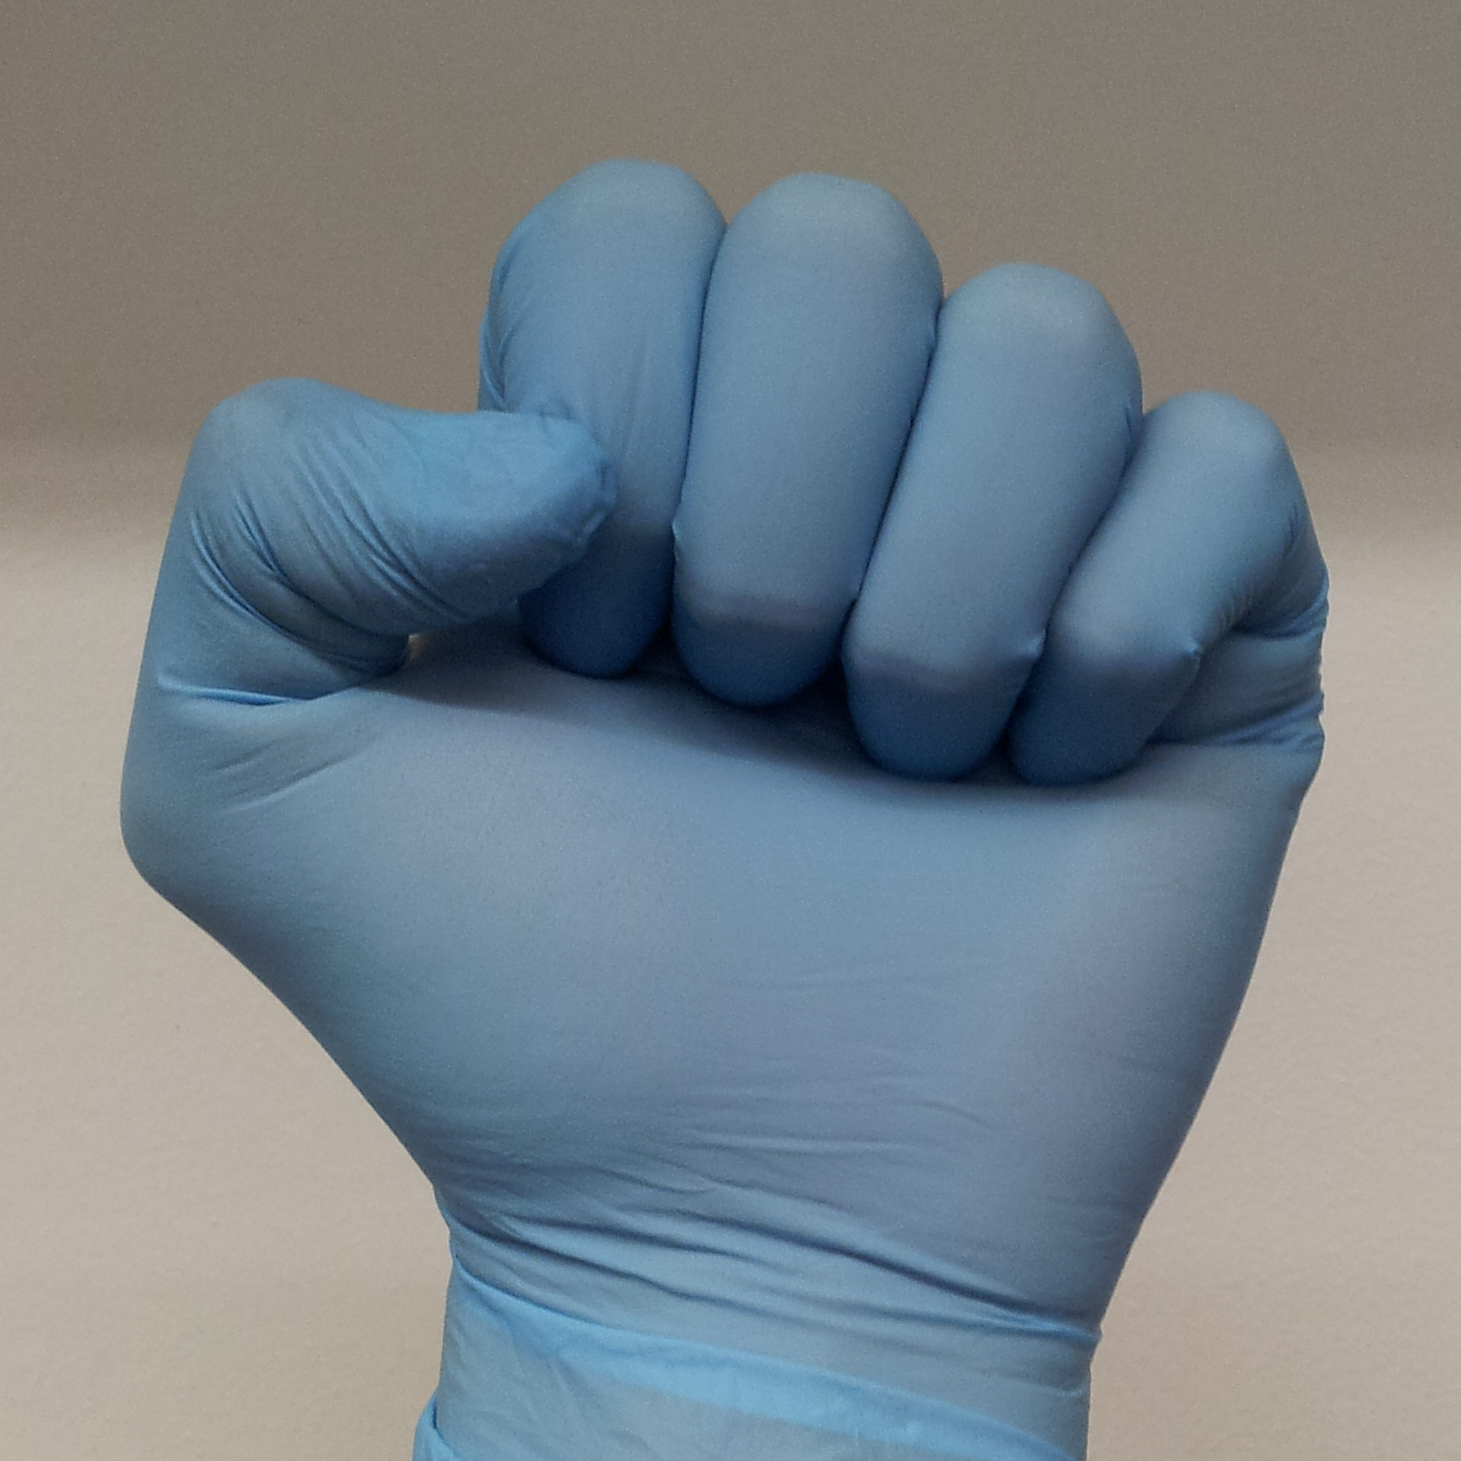
\includegraphics[width=0.23 \textwidth]{fig/gesture2.png}
%\\
%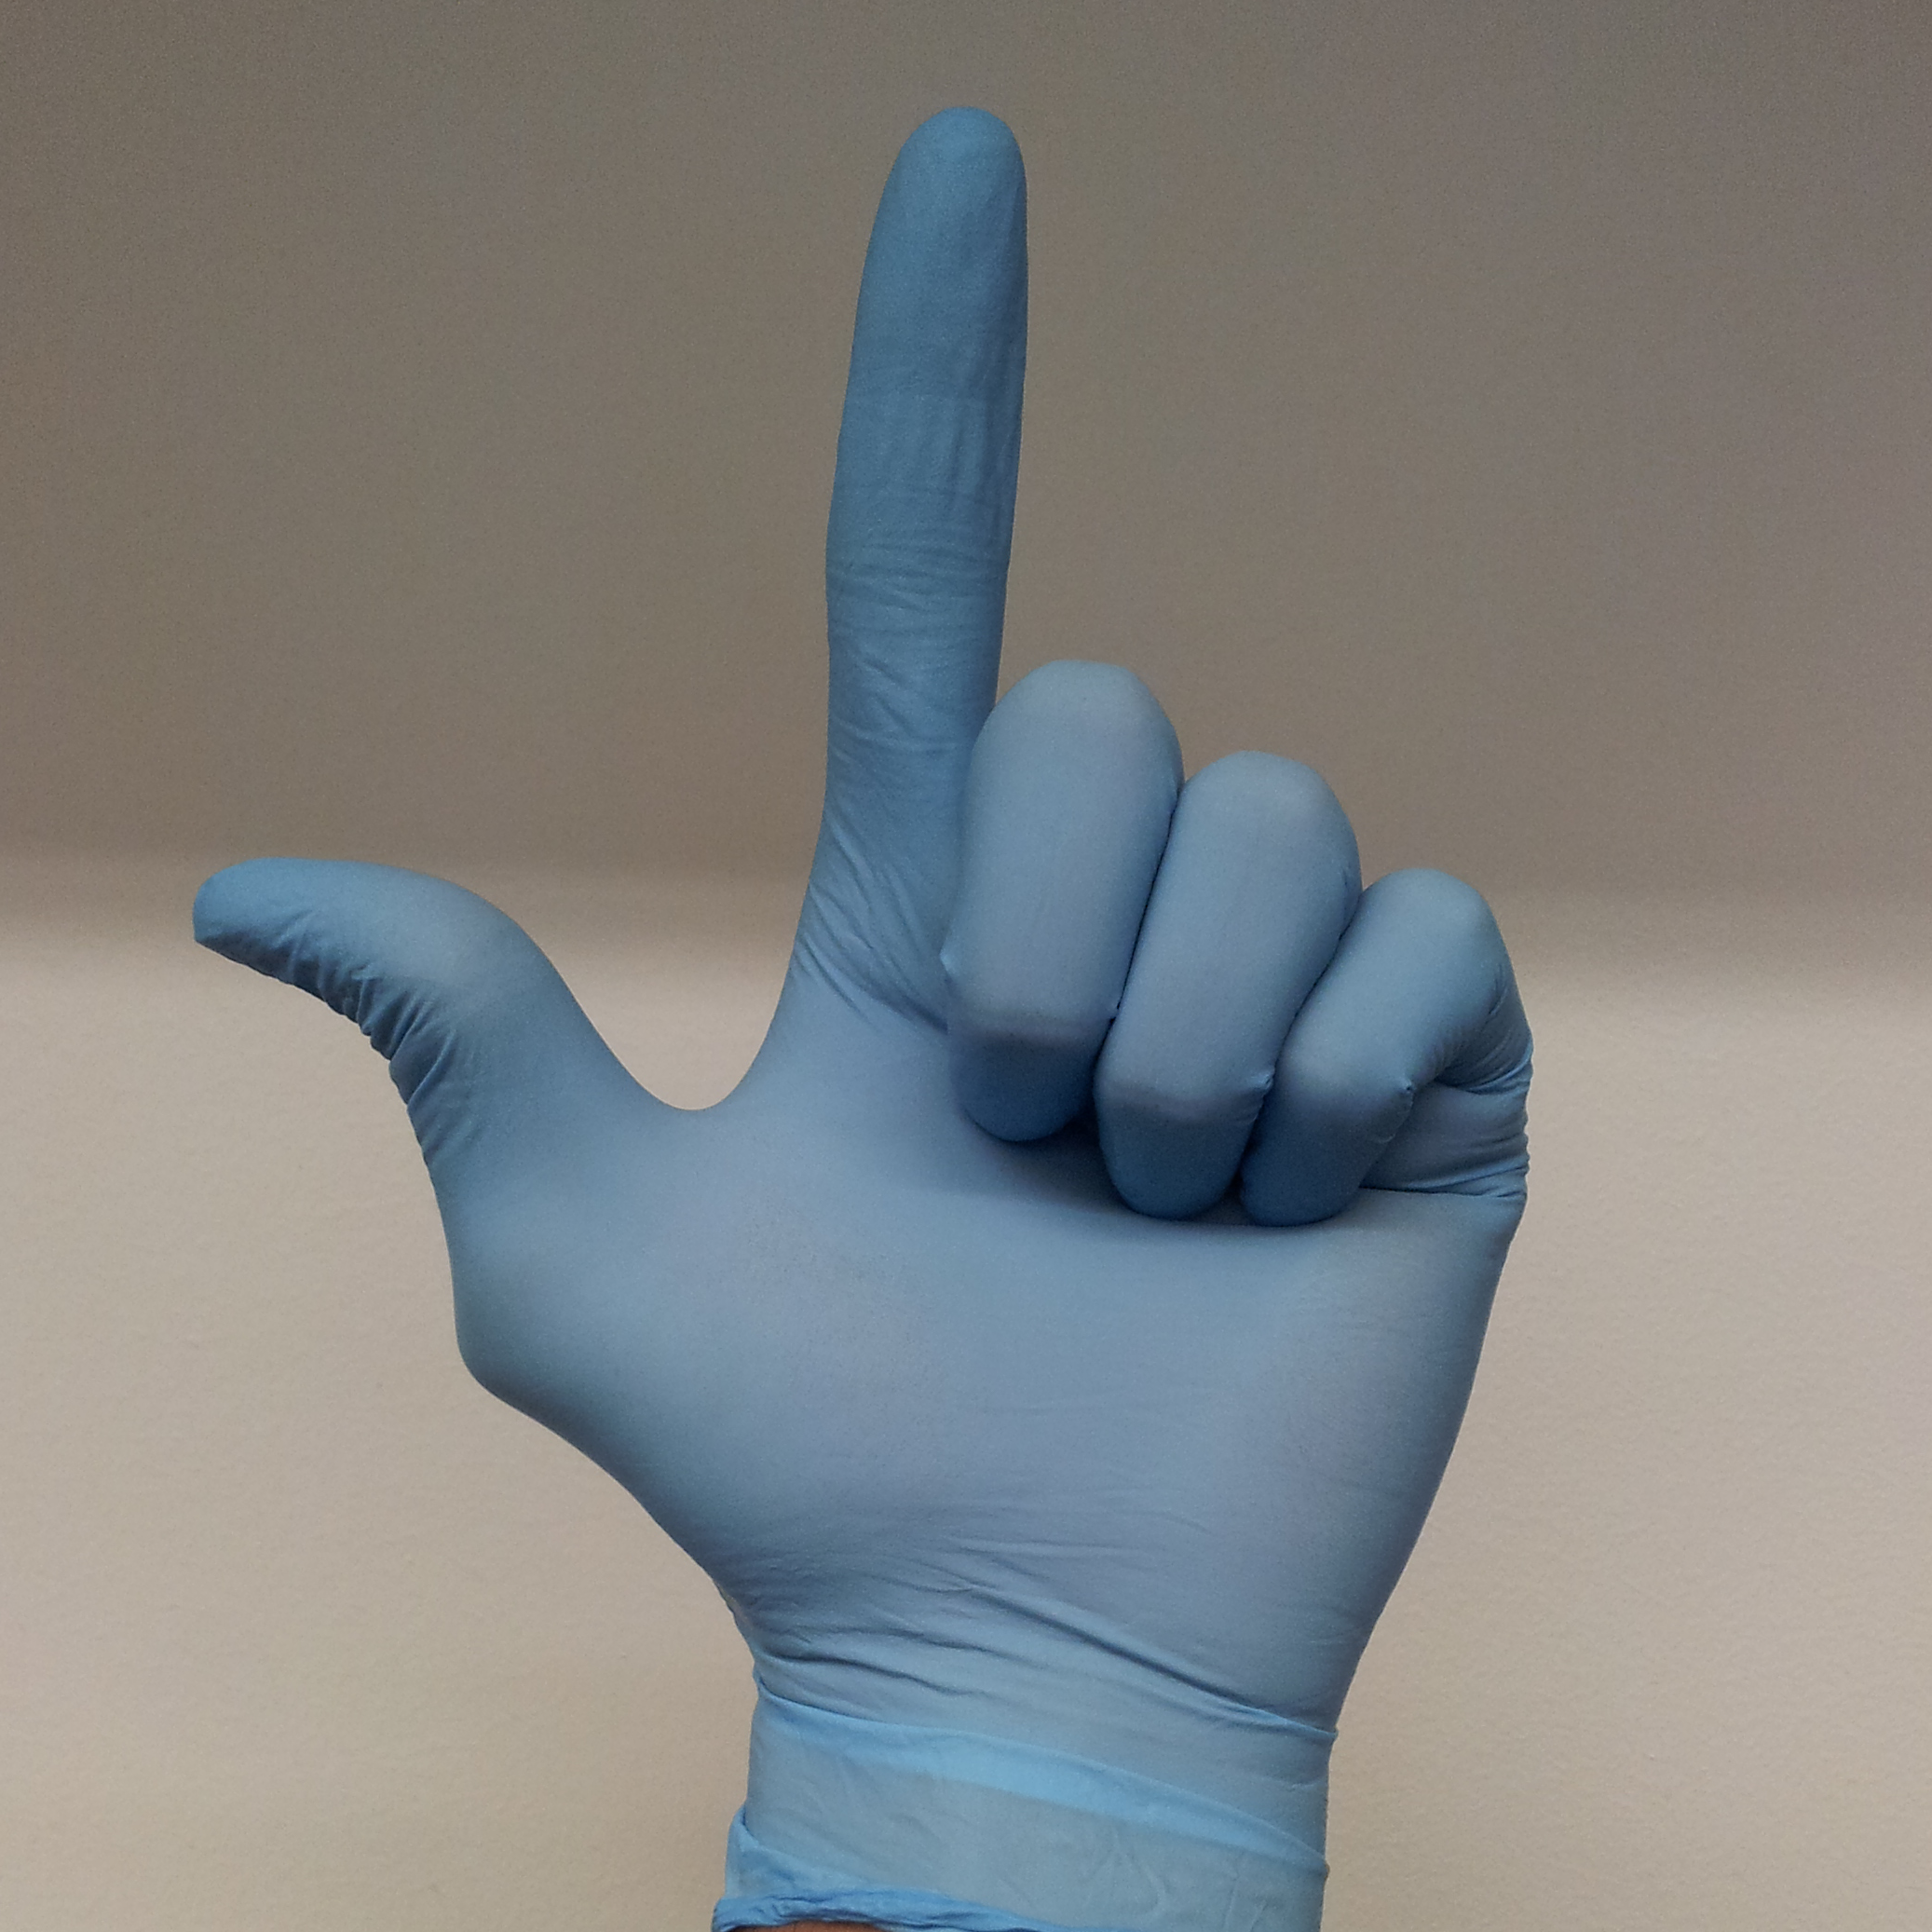
\includegraphics[width=0.23 \textwidth]{fig/gesture3.png}
%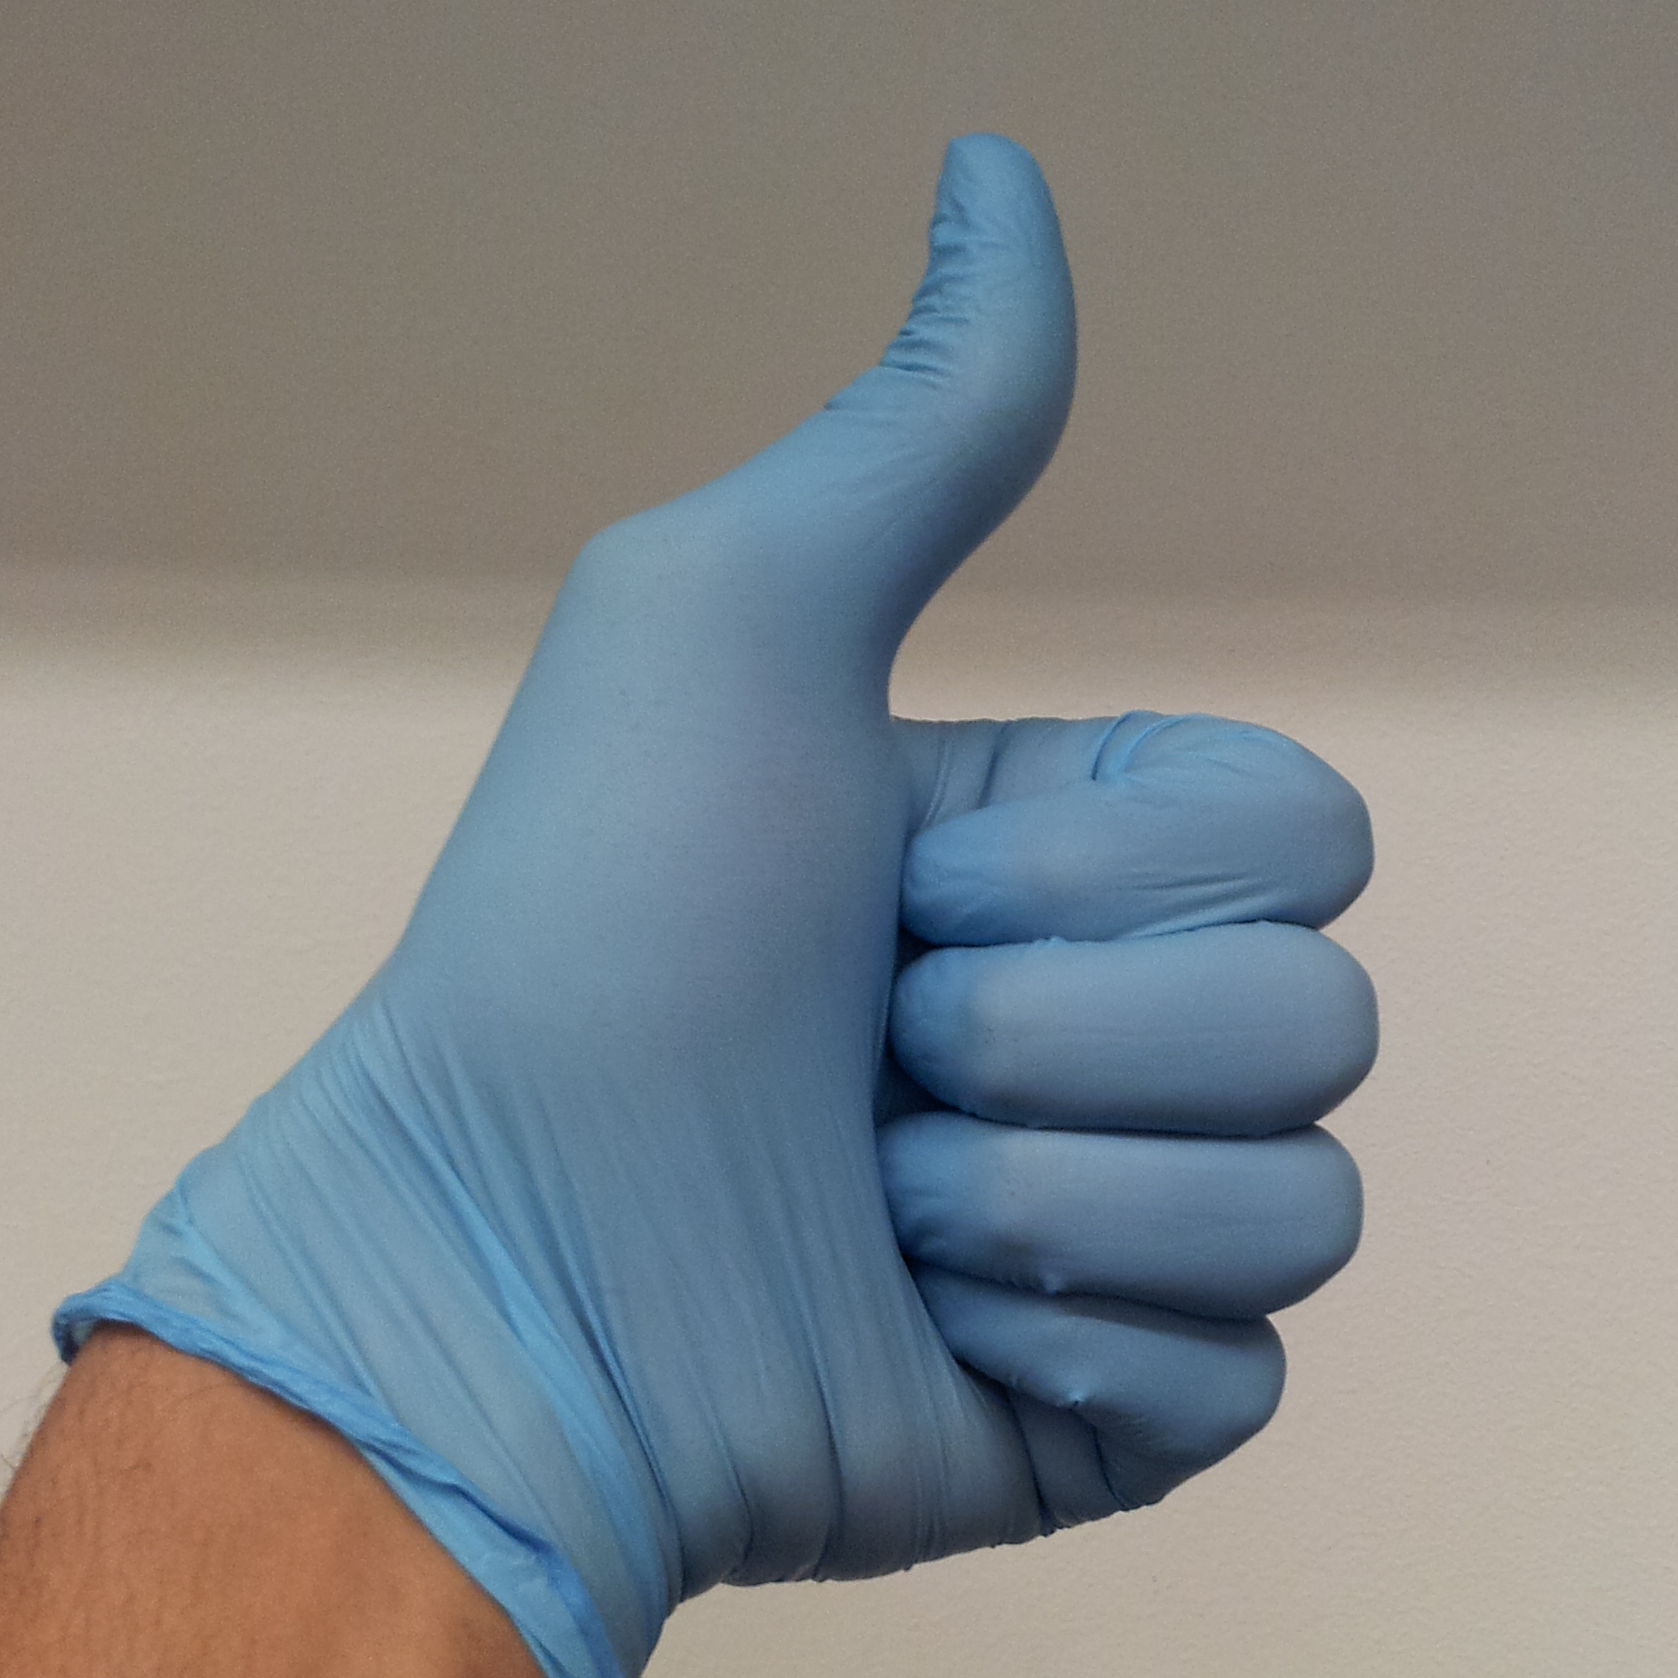
\includegraphics[width=0.23 \textwidth]{fig/gesture4.png}
\end{center}
\caption{An example of four gestures. Each gesture represent a label of every pixel that belongs to the glove.  
%seen above were chosen because of their potential applicability to data visualization interaction systems. For example, the first figure may be used to instruct the application to translate the visualization along with the hand. The second image could lock the image in place while the other hand forms gestures.
}
\label{fig:gestures}
\end{figure}


We devised two different techniques of labeling each pixel. The first technique, shown in the left image of Figure~\ref{fig:gloves}, is to differentiate all pixels in the hand from the background. When training the system, we train one gesture at a time and classify a pixel on the hand as belonging to that gesture and classify any pixel not on the hand as part of the background. We trained four gestures using this approach yielding a total of five labels. An example of the gestures can be seen in Figure~\ref{fig:gestures}. The second technique is shown in the right image of Figure~\ref{fig:gloves}. In this technique each finger is labeled separately. Therefore each pixel can have a total of seven labels - six for the hand, and one for the background.

We also use other techniques to simplify labeling such as cropping and ignoring far away pixels via the depth information.